% Chapter Template

\chapter{Ensayos y resultados} % Main chapter title

\label{Chapter4} % Change X to a consecutive number; for referencing this chapter elsewhere, use \ref{ChapterX}

%----------------------------------------------------------------------------------------
%	SECTION 1
%----------------------------------------------------------------------------------------
En este capítulo se explica la metodología de pruebas aplicada tanto a los componentes individuales como al sistema implementado para finalizar con una comparación con el estado del arte.


\section{Banco de pruebas}
\label{sec:Banco de pruebas}
%
%La verificación del correcto funcionamiento de los módulos que componen el sistema se realizó mediante una maqueta que represente en escala reducida al invernadero del cliente.
%El modelo cuenta con una bomba de agua conectada a tres válvulas para simular hasta tres circuitos de riego.
%Para el armado se utilizaron mangueras y conexiones neumáticas de aluminio de acople rápido como muestra la figura \ref{fig:pump}   
%El proceso de construcción de la maqueta se muestra en la figura \ref{fig:invernadero}, allí se observa la implementación de dos circuitos de riego independientes para diferentes clases de macetas y se configuró un tercer circuito cerrado de agua para pruebas de accionamiento de bomba y válvula para evitar desperdicios durante las fases de calibración.
%
%
%\begin{figure}[h]
%	\centering
%	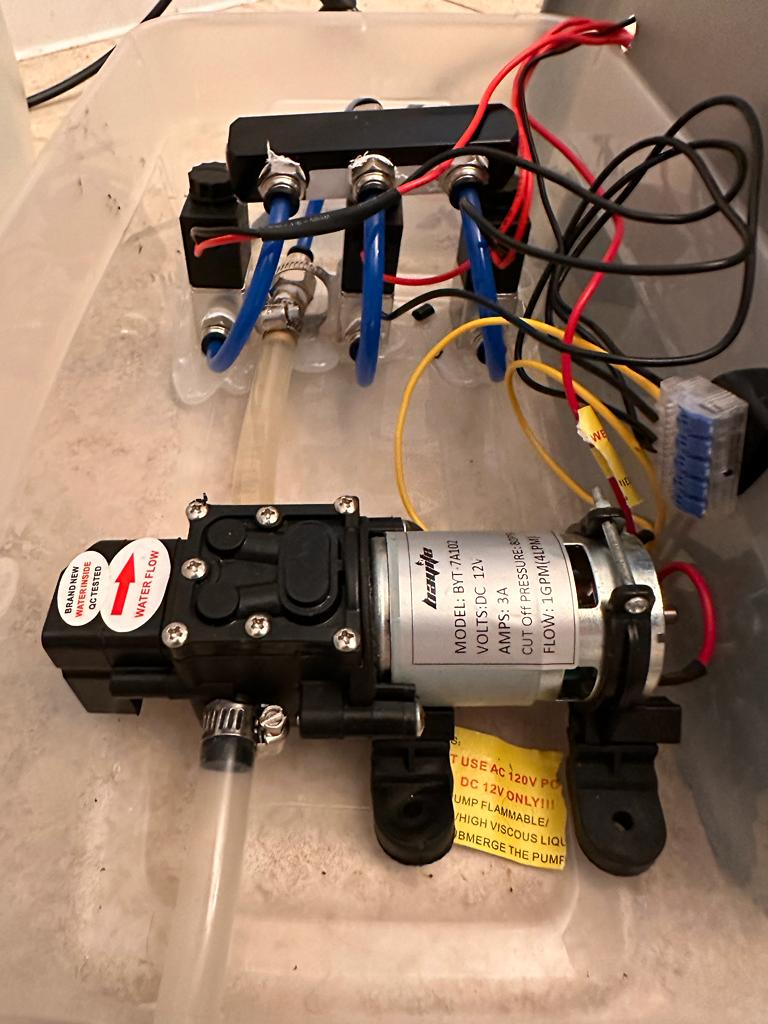
\includegraphics[width=0.5\textwidth]{./Figures/chapter4/pump_2.jpg}
%	\caption[Conexión de bomba y válvulas]{Conexión de bomba y válvulas.}
%	\label{fig:pump}
%\end{figure}
%
%\begin{figure}[!htpb]
%     \centering
%     \begin{subfigure}[b]{0.45\textwidth}
%		\centering
%		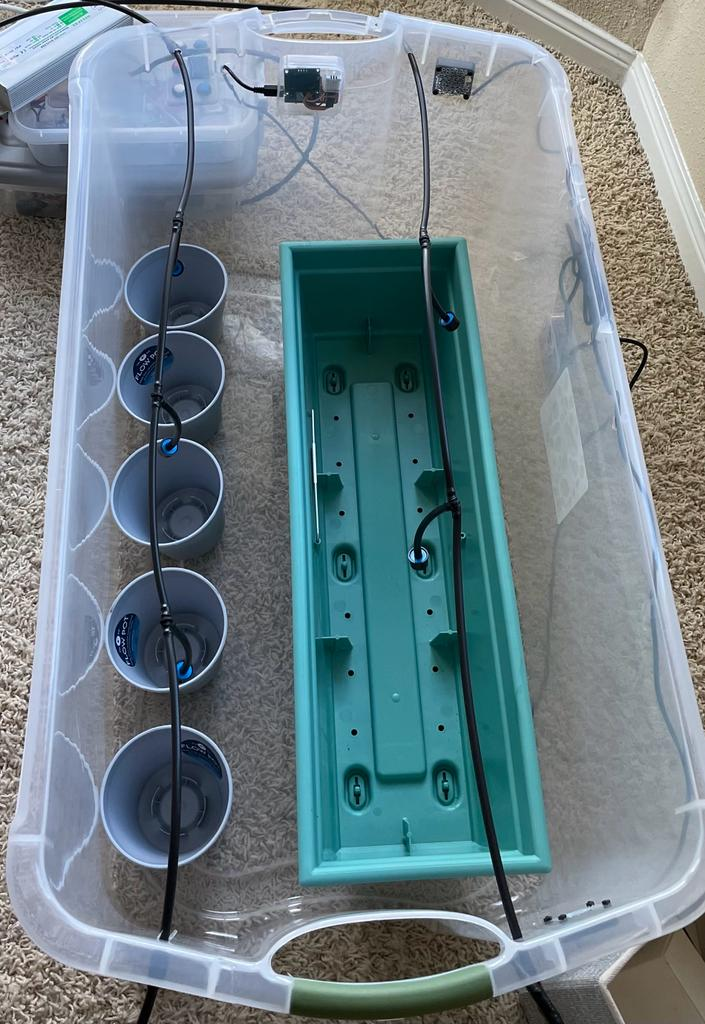
\includegraphics[width=0.70\textwidth]{./Figures/chapter4/Invernadero1.jpg}
%		\caption{Armado de mangueras de riego.}
%		\label{fig:gh1}
%     \end{subfigure}
%     \hfill
%     \begin{subfigure}[b]{0.45\textwidth}
%	    \centering
%		 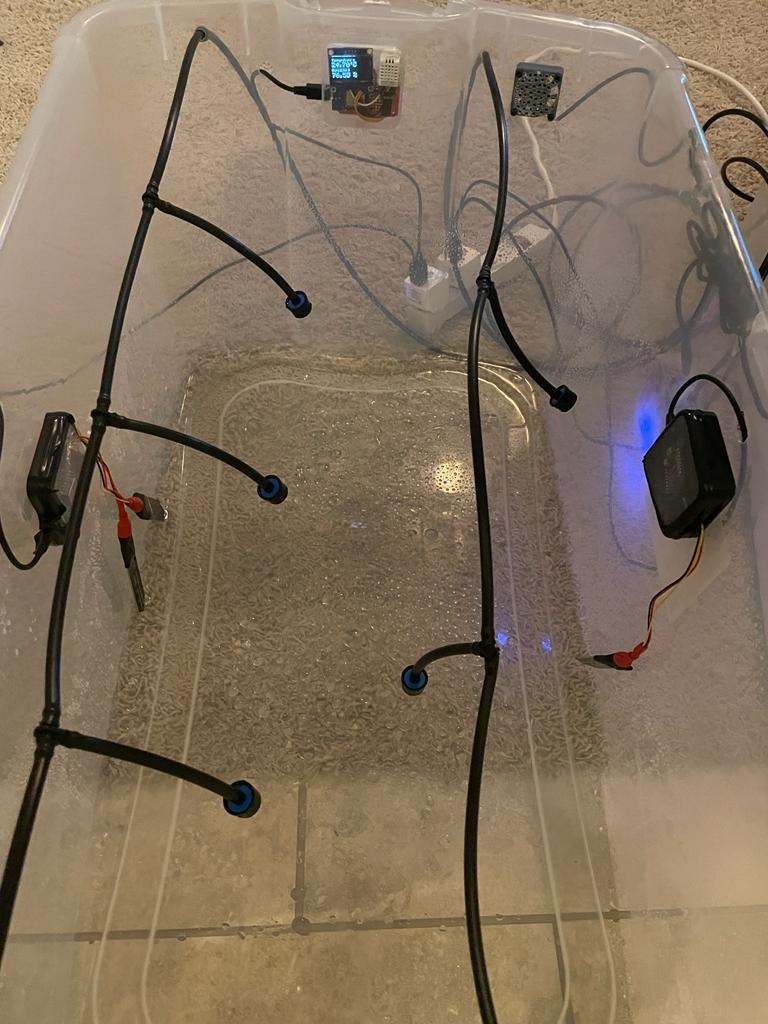
\includegraphics[width=0.75\textwidth]{./Figures/chapter4/Invernadero2.jpg}
%		\caption{Pruebas de riego.}
%		\label{fig:gh2}
%     \end{subfigure}
%     \hfill	
%	 \begin{subfigure}[b]{0.45\textwidth}
%		\centering
%		\includegraphics[width=0.60\textwidth]{./Figures/chapter4/Invernadero3.jpg}
%		\caption{Ensamble general.}
%		\label{fig:gh3}
%     \end{subfigure}
%     \hfill
%%          \begin{subfigure}[b]{0.45\textwidth}
%%		\centering
%%		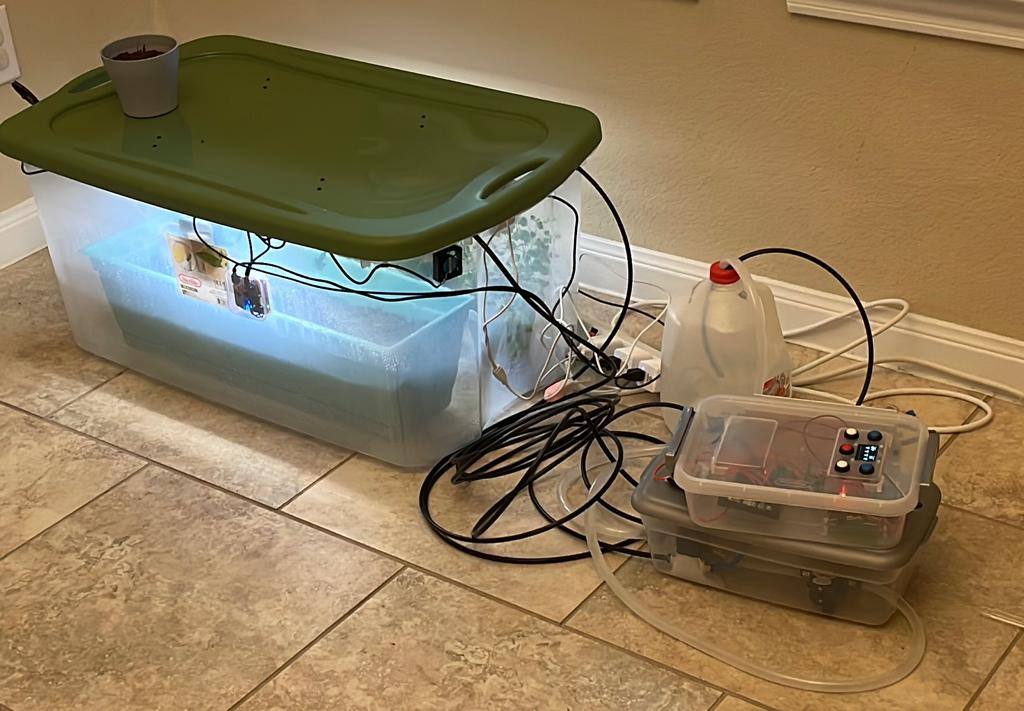
\includegraphics[width=0.90\textwidth]{./Figures/chapter4/Invernadero4.jpg}
%%		\caption{Modelo terminado.}
%%		\label{fig:gh4}
%%     \end{subfigure}
%%     \hfill
%     \begin{subfigure}[b]{0.45\textwidth}
%	    \centering
%		 \includegraphics[width=0.80\textwidth]{./Figures/chapter4/Invernadero5.jpg}
%		\caption{Modelo terminado.}
%		\label{fig:gh5}
%     \end{subfigure}
%     \hfill	
%
%        \caption[Modelo de pruebas del invernadero]{Modelo de pruebas del invernadero.}
%        \label{fig:invernadero}
%\end{figure}
%
%La tabla \ref{tab:herramientas} detalla las diferentes herramientas empleados para la configuración y validación de requerimientos sobre el sistema:
%
%
%
%\begin{table}[h]
%\centering
%\caption[Herramientas empleadas para las pruebas]{Herramientas empleadas para las pruebas.}
%
%%\begin{tabular}{ll} } 
%\begin{tabularx}{\textwidth}{sb}  
%\toprule
%\textbf{Recurso} & \textbf{Función}\\
%
%\midrule
%				&	\tabitem Instalación y configuración de Thingsboard. \\
%Computadora      &   \tabitem Desarrollo y carga del firmware en módulos. \\
%                &   \tabitem Pruebas de acceso y concurrencia al sistema. \\
%Teléfono celular	& Pruebas de acceso y concurrencia al sistema.\\
%Pistola de calor	& Pruebas de control de temperatura. \\
%Recipientes y tierra fértil	&	Calibración de sensores de humedad del suelo.\\ 
%Protoboard y leds	& Pruebas sobre módulos actuadores.\\
%\bottomrule
%\hline
%\end{tabularx}
%\label{tab:herramientas}
%\end{table}

\section{Pruebas unitarias}
\label{sec:Pruebas unitarias}


\section{Pruebas de sistema}
\label{sec:Pruebas de sistema}



\section{Comparativa con el estado de arte}
\label{sec:Comparativa con el estado de arte}